\documentclass[notitlepage, reprint, nofootinbib]{revtex4-1}
\usepackage[utf8]{inputenc}

% Mathematics and symbols:
\usepackage{amsmath, gensymb, amsthm, physics, mhchem}
% Figures:
\usepackage{tikz, graphicx}
\usepackage[caption=false]{subfig}

% Other:
\usepackage{hyperref}

\hypersetup{
    colorlinks=true,
    linkcolor=purple,
    filecolor=magenta,      
    urlcolor=purple,
}

\usepackage{algorithm}
\usepackage{algpseudocode}


% Document formatting 
\setlength{\parskip}{1mm}
\setlength{\parindent}{0mm}


%\renewcommand{\thesubsubsection}{\alph{subsubsection})}


\begin{document}
\title{Disease Modeling \\[2mm] \normalsize{FYS3150 - Project 5}}
\author{Frida Larsen}

\begin{abstract}
This report aims to study the SIR-model of epidemiology using two different approaches; a direct numerical integration of the partial differential equations and a discrete method based on Monte Carlo techniques. The basic SIR-model is expanded to include vital dynamics, seasonal variation and vaccination. Both the direct integration and the Monte Carlo simulation successfully incorporates these elements. Whereas the Monte Carlo method reflects important realistic elements, the direct approach is easier to interpret. Furthermore, due to random effects, large scale patterns appear slower for the Monte Carlo method than for the direct integration. 
\end{abstract}

\maketitle

\section{Introduction}
Epidemiology is the study of the health status and disease prevalence in a population.\cite{Epidemiologi} Understanding how diseases spread and develop over time is crucial in order to control their expanse and establish preventative measures. \\[2mm]
The aim of this report is to study the SIR-model of epidemiology. Two models will be implemented; a differential model and a discrete model. The first will be solved using a fourth order Runge-Kutta shceme, while the latter will be solved using a Monte Carlo method. We will compare the two models in terms of features and quality.\\[2mm]
All relevant code may be found in the GitHub repository 'FYS3150-Computational-Physics'\footnote{\href{GitHub Repository}{https://github.com/fridalarsen/FYS3150-Computational-Physics}} under the Project5 folder. This folder also includes a Figures folder, which holds all the figures presented in this text and produced during the project. The SIR-model and its solutions are implemented as a class which may be found in the '\texttt{improved\_SIR.py}'-program.

\section{Theory: The SIR-model}
The SIR-model is a compartmental model. Such models describe how individuals move between groups, or compartments, in a population. These models are frequently used in order to simulate infectious diseases. \\[2mm]
In the SIR-model, every individual in a population of $N$ people are sorted into three groups according to their status related to a specific disease: 
\begin{itemize}
	\item Susceptible individuals (S): Those without immunity to the disease
	\item Infected individuals (I): Those currently infected with the disease 
	\item Recovered individuals (R): Those who have been infected in the past and have developed immunity 
\end{itemize}
The flow of people moving between each group is described by the rate of transmission ($a$), the rate of recovery ($b$) and the rate of immunity loss ($c$). See figure \ref{sketch} for an illustration. 
\begin{figure}[h!]
	\centering
	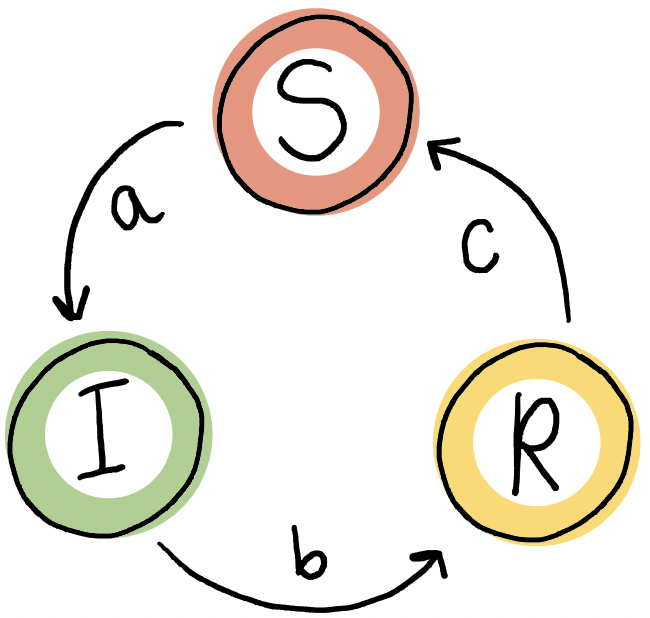
\includegraphics[width=0.2\textwidth]{../Figures/SIR-model_illustration.png}
	\caption{An illustration of the SIR-model groups and transition rates.}
	\label{sketch}
\end{figure}
\subsection{The basic SIR-model}
In the basic SIR-model, we assume that the disease in question is a non-deadly disease and that the time scale of this epidemic is smaller than an average person's lifetime. The population should thus remain constant during the period:	
\begin{equation}\label{SIR-eq}N=S(t)+I(t)+R(t)\end{equation}
Using this, we get the following set of differential equations:
\begin{align}
	S' &= cR-\frac{aSI}{N}\label{SIR1_S}\\
	I' &= \frac{aSI}{N}-bI\label{SIR1_I}\\
	R' &= bI - cR \label{SIR1_R}
\end{align}
\newpage
\subsection{The improved SIR-model}
The basic SIR-model provides a good picture of a simple epidemic. However, it can be improved in order to allow us to study more complex diseases. Firstly, some diseases spread over long stretches of time so that the population change must be taken into account. In addition, we want to be able to include deadly diseases.\\[2mm]
By introducing a birth rate ($e$), death rate ($d$) and disease death rate ($d_I$) we get the following set of differential equations: 
\begin{align}
	S' &= cR-\frac{aSI}{N} - dS + eN\label{SIR2_S}\\
	I' &= \frac{aSI}{N}-bI - dI- d_II\label{SIR2_I}\\
	R' &= bI - cR - dR\label{SIR2_R}
\end{align}
Note that this project will not include passive immunity. We will assume that every newborn child is susceptible to the disease.\\[2mm]
Furthermore, we wish to include so-called seasonal diseases that vary with time. Although there are many mechanisms behind this seasonal variation\cite{seasonal}, the variation itself can be modelled as a fluctuation in the transmission rate, $a$. We set
\begin{equation}a(t)=A\cos(\omega t)+a_0,\end{equation}
where $a_0$ is the average transition rate, $A$ is the maximum deviation from $a_0$ and $\omega$ is the frequency of the fluctuation.\\[2mm]
Ever since the smallpox vaccine was invented by Edward Jenner in the late 1700's\cite{vaccination}, vaccination has been an incomparable tool for eradicating and treating diseases. In our framework, vaccination allows people to move directly from susceptible to recovered. By introducing a vaccination rate ($f$), we get the following set of differential equations:
\begin{align}
	S' &= cR-\frac{aSI}{N} - fS\\
	I' &= \frac{aSI}{N}-bI\\
	R' &= bI - cR + fS
\end{align}
Finally, by combining the differential equations with vital dynamics and the equations for vaccination, we get a combined model:
\begin{align}
	S' &= cR-\frac{aSI}{N} - dS + eN - fS\\
	I' &= \frac{aSI}{N}-bI - dI- d_II\\
	R' &= bI - cR - dR + fS
\end{align}

\section{Method}
There are several approaches for implementing the model developed above. We will focus on two solution methods, namely direct numerical integration, using the fourth order Runge-Kutta scheme, and a Monte Carlo method.
\subsection{Fourth Order Runge-Kutta}
The algorithm for using fourth order Runge-Kutta to find the next step of a discretized differential equation is given by\cite{Langtangen}
\begin{algorithm}[H]
	\caption{4th order Runge-Kutta for finding the next step}
	\begin{algorithmic}[1]
		\State $K_1=hf(t_i, y_i)$
		\State $K_2 = hf(t_i+h/2, y_i+k_1/2)$
		\State $K_3 =hf(t_i+h/2, y_i+k_2/2)$ 
		\State $K_4 = hf(t_i+h, y_i+k_3)$
		\State $y_{i+1}=y_i+1/6(K_1+2K_2+2K_3+K_4)$
	\end{algorithmic}
\end{algorithm}
where $h$ is the time step, so that $t_i=t_{i-1}+h$.

\subsection{Monte Carlo}
The differential equations used to model the population are inherently continuous, however this is not true for a real population. 
In order to emulate a discrete population, we can use the idea of randomness in Monte Carlo methods to model discrete jumps between S, I and R. \\[2mm] 
From the original differential equations (equations \ref{SIR1_S}-\ref{SIR1_R}) we see that, per time step, approximately $(\Delta t\frac{aSI}{N})$ people move from S to I. Similarly, about $(\Delta t\ bI)$ move from I to R and roughly $(\Delta t\ cR)$ move from R to S.\\[2mm]
By assuming that $\Delta t$ is small enough so that no more than 1 person moves from group to another, we get  
\begin{align}
	\text{max}\Big\{\Delta t\frac{aSI}{N}\Big\}=\frac{aN}{4}\Delta t\overset{!}{=}1\\
	\text{max}\Big\{\Delta t\ bI\Big\}=bN\Delta t\overset{!}{=}1\\
	\text{max}\Big\{\Delta t\ cR\Big\}=cN\Delta t\overset{!}{=}1
\end{align}
By solving for the time step we get three options, namely
\begin{equation}\label{time_steps}\Delta t=\Big\{\frac{4}{aN},\frac{1}{bN},\frac{1}{cN}\Big\}.\end{equation}
The time step used for each Monte Carlo iteration is whichever of these is the smallest during that iteration. We can now formulate a set of transition probabilities describing the (basic) system:
\begin{align}
	P(S\rightarrow I)&=\frac{aSI}{N}\Delta t\label{prob1}\\
	P(I\rightarrow R)&=bI\Delta t\\
	P(R\rightarrow S) &= cR\Delta t
\end{align}
The probabilities including seasonal variation are the same as the above, but with a variable $a$, $a(t)$.\\[2mm]
In order to include vaccination, we must add a third option, as some individuals will move directly from being susceptible to being recovered. We have
\begin{align}
	P(S\rightarrow R)&=fS\Delta t\label{prob2},
\end{align}
where $f$ can be a constant or a function, $f(t)$.\\[2mm]
For each cycle, a random number is drawn. The number determines which of the moves to perform or if no moves should be performed at all.\\[2mm] 
We get the following algorithm for determining the move: 
\begin{algorithm}[H]
	\caption{Monte Carlo cycle}
	\begin{algorithmic}[1]
		\State Calculate time step by taking the minimum of equation \ref{time_steps}.
		\State Compute transition probabilities by equations \ref{prob1}-\ref{prob2}.
		\State Draw two random numbers, $r$ and $j$, where $j$ corresponds to the index of a list containing all possible transitions.
		\State Find transition corresponding to the drawn $j$.
		\If{$r<P_j$}
			\State Accept move. 
		\Else
			\State Deny move.
		\EndIf
	\end{algorithmic}
\end{algorithm}
After determining the move that is to happen, we need to update the population in terms of births and deaths (if vital dynamics are included). From equations \ref{SIR2_S}-\ref{SIR2_R} we get 
\begin{align}
	P(\text{birth})&=eN\Delta t\label{birth}\\
	P(\text{death in S}) &= dS\Delta t \\
	P(\text{death in I}) &= (d+d_1)I\Delta t\\
	P(\text{death in R}) &= dR\Delta t\label{deathR}
\end{align}
We get the following algorithm for population change:
\begin{algorithm}[H]
	\caption{Population change}
	\begin{algorithmic}[1]
		\State Compute probabilities for population change from equations \ref{birth}-\ref{deathR}.
		\State Draw four random numbers; $r_1$, $r_2$, $r_3$ and $r_4$.
		\If{$r_1 < P(\text{birth})$}
			\State Add new susceptible individual into population. 
		\ElsIf {$r_2<P(\text{death in S})$}
			\State Remove a susceptible individual. 
		\ElsIf{$r_3<P(\text{death in I})$}
			\State Remove an infected individual.
		\ElsIf{$r_4<P(\text{death in R})$}
			\State Remove a recovered individual.
		\EndIf
	\end{algorithmic}
\end{algorithm}

\subsection{Scenarios}
For this project we will focus on five different scenarios. \\[2mm]
\begin{enumerate}
	\item We will begin by comparing four different populations in terms of rates of recovery. The population parameters are presented in table \ref{RK4_populations}. The next four scenarios focus on population A.
	\item This scenario introduces vital dynamics using a birth rate of $e=0.3$, a (natural) death rate of $d=0.2$ and a disease death rate of $d_I=0.55$.  
	\item This scenario introduces seasonal variation with $$a(t)=3\cos(0.5t) + 4.$$
	\item This scenario introduces vaccination with $$f(t)=\begin{cases}0, \quad &\text{for $t < 5$} \\ 1, \quad &\text{for $t>5$}\end{cases}$$
	\item This scenario combines vital dynamics, seasonal variation and vaccination. The birth rate was set to $e=0.3$, the (natural) death rate to $d=0.3$ and the disease death rate to $d_I=0.55$. Vaccination rate was set as $$f(t)=\begin{cases}0, \quad &\text{for $t < 5$} \\ 0.2, \quad &\text{for $t>5$}\end{cases}$$ Seasonal variation was set as $$a(t)=3\cos(0.5t) + 4.$$
\end{enumerate}
\begin{table}[]
\centering
\begin{tabular}{|c|c|c|c|c|}
\hline
 & A & B & C & D \\ \hline
a & 4 & 4 & 4 & 4 \\ \hline
b & 1 & 2 & 3 & 4 \\ \hline
c & 0.5 & 0.5 & 0.5 & 0.5 \\ \hline
\end{tabular}
\caption{Population parameters for four different populations.}
\label{RK4_populations}
\end{table}
\newpage
\section{Results}
Figures \ref{RK4_A}, \ref{RK4_B}, \ref{RK4_C} and \ref{RK4_D} show the time development of susceptible, infected and recovered individuals in populations A, B, C and D respectively for scenario 1. The corresponding simulations done using Monte Carlo are presented in figures \ref{MC_A}, \ref{MC_B}, \ref{MC_C} and \ref{MC_D}.\\[2mm]
The results of scenario 2 are presented in figures \ref{RK4_vr} and \ref{MC_vr}. The plots show the development of the population size, in addition to the usual susceptible, infected and recovered categories.\\[2mm]
The results of scenario 3 are presented in figures \ref{RK4_sv} and \ref{MC_sv}.\\[2mm]
The results of scenario 4 are presented in figures \ref{RK4_vacc} and \ref{MC_vacc}. The dashed line indicates the start of vaccination. 
Finally, the results of scenario 5 are presented in figures \ref{RK4_combo} and \ref{MC_combo}. Again, the dashed lines indicate the start of vaccination.
\begin{figure}[h!]
	\centering
	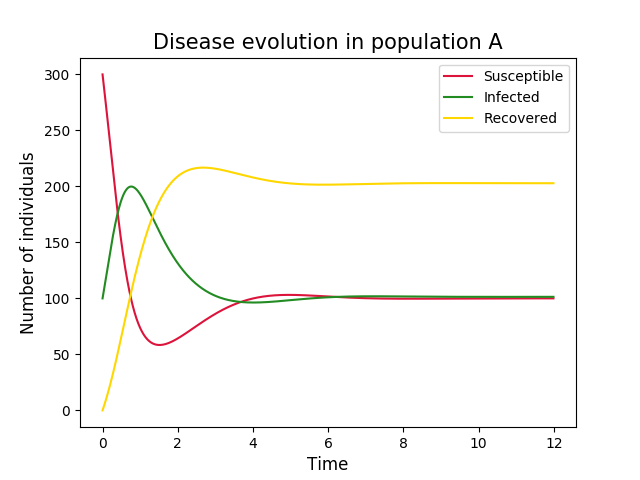
\includegraphics[width=0.45\textwidth]{../Figures/RK4_population_A}
	\caption{Time evolution of number of susceptible, infected and recovered individuals in population A, computed using Runge-Kutta 4.}
	\label{RK4_A}
\end{figure}
\begin{figure}[h!]
	\centering
	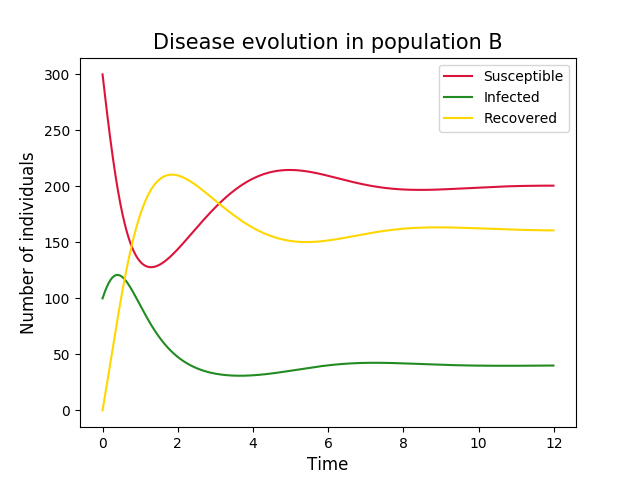
\includegraphics[width=0.45\textwidth]{../Figures/RK4_population_B}
	\caption{Time evolution of number of susceptible, infected and recovered individuals in population B, computed using Runge-Kutta 4.}
	\label{RK4_B}
\end{figure}
\begin{figure}[h!]
	\centering
	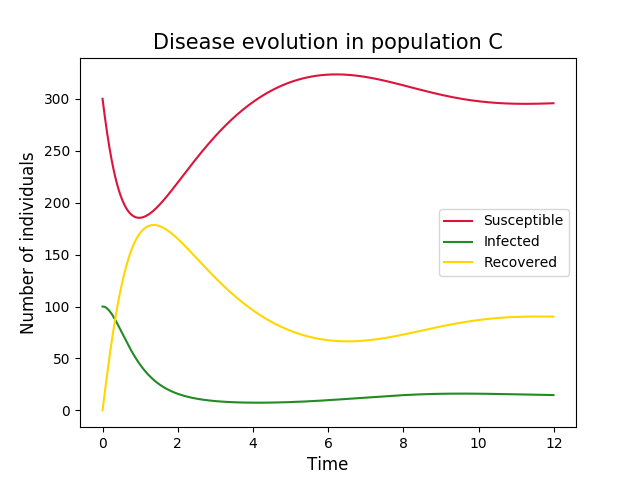
\includegraphics[width=0.45\textwidth]{../Figures/RK4_population_C}
	\caption{Time evolution of number of susceptible, infected and recovered individuals in population C, computed using Runge-Kutta 4.}
	\label{RK4_C}
\end{figure}
\begin{figure}[h!]
	\centering
	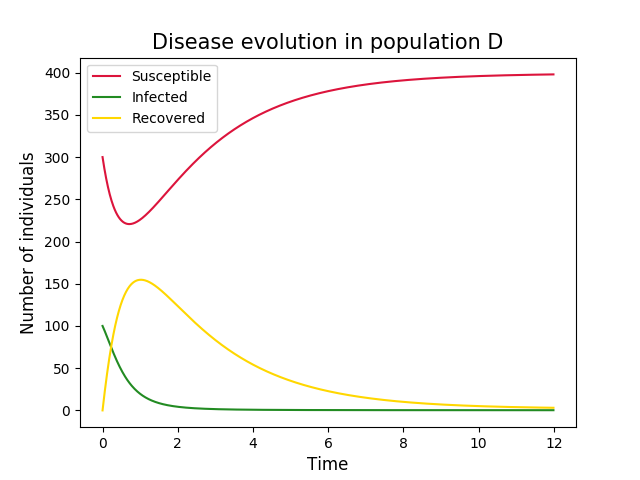
\includegraphics[width=0.45\textwidth]{../Figures/RK4_population_D}
	\caption{Time evolution of number of susceptible, infected and recovered individuals in population D, computed using Runge-Kutta 4.}
	\label{RK4_D}
\end{figure}
\begin{figure}
	\centering
	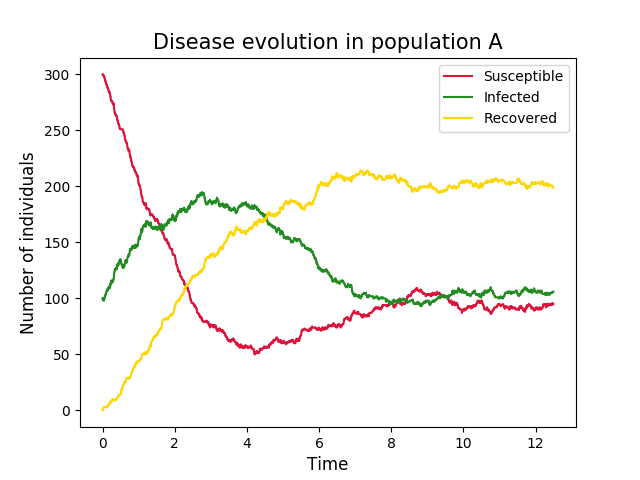
\includegraphics[width=0.45\textwidth]{../Figures/MC_population_A}
	\caption{Time evolution of number of susceptible, infected and recovered individuals in population A, computed using a Monte Carlo method.}
	\label{MC_A}
\end{figure}
\begin{figure}
	\centering
	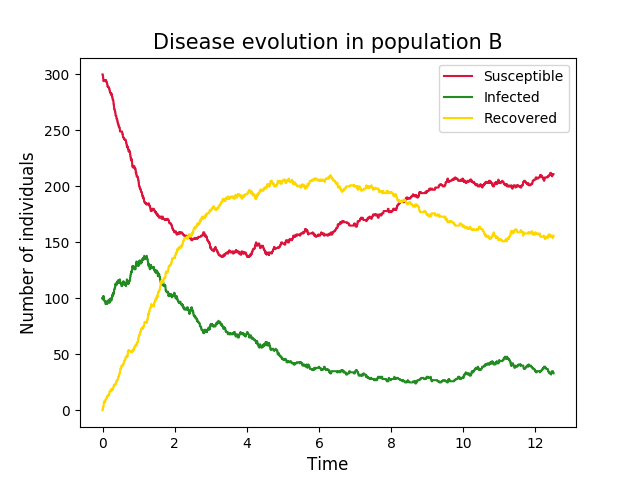
\includegraphics[width=0.45\textwidth]{../Figures/MC_population_B}
	\caption{Time evolution of number of susceptible, infected and recovered individuals in population B, computed using a Monte Carlo method.}
	\label{MC_B}
\end{figure}
\begin{figure}
	\centering
	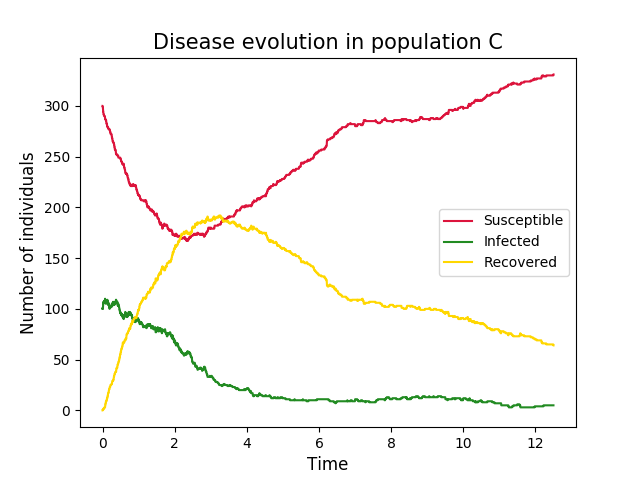
\includegraphics[width=0.45\textwidth]{../Figures/MC_population_C}
	\caption{Time evolution of number of susceptible, infected and recovered individuals in population C, computed using a Monte Carlo method.}
	\label{MC_C}
\end{figure}
\begin{figure}
	\centering
	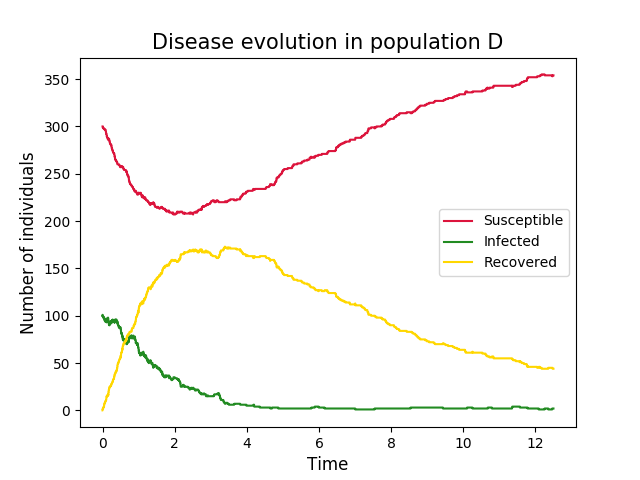
\includegraphics[width=0.45\textwidth]{../Figures/MC_population_D}
	\caption{Time evolution of number of susceptible, infected and recovered individuals in population D, computed using a Monte Carlo method.}
	\label{MC_D}
\end{figure}
\begin{figure}
	\centering
	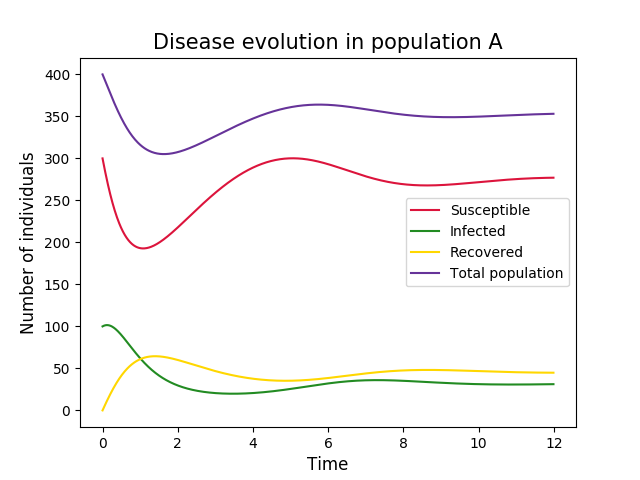
\includegraphics[width=0.45\textwidth]{../Figures/RK4_popA_vr}
	\caption{Time evolution of population A with vital dynamics, computed using RK4.}
	\label{RK4_vr}
\end{figure}
\begin{figure}
	\centering
	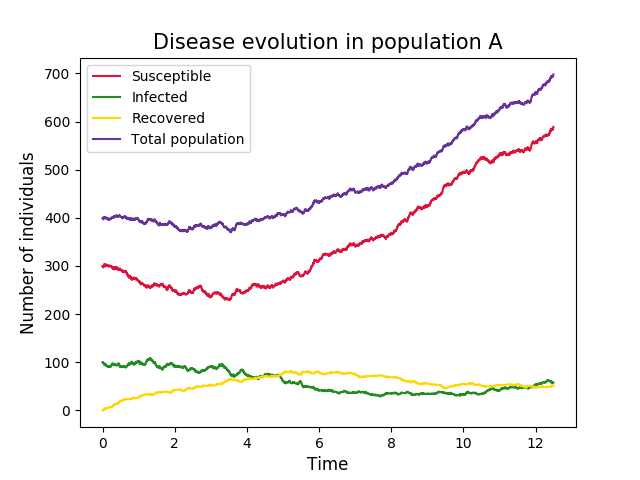
\includegraphics[width=0.45\textwidth]{../Figures/MC_popA_vr}
	\caption{Time evolution of population A with vital dynamics, computed using Monte Carlo.}
	\label{MC_vr}
\end{figure}
\begin{figure}
	\centering
	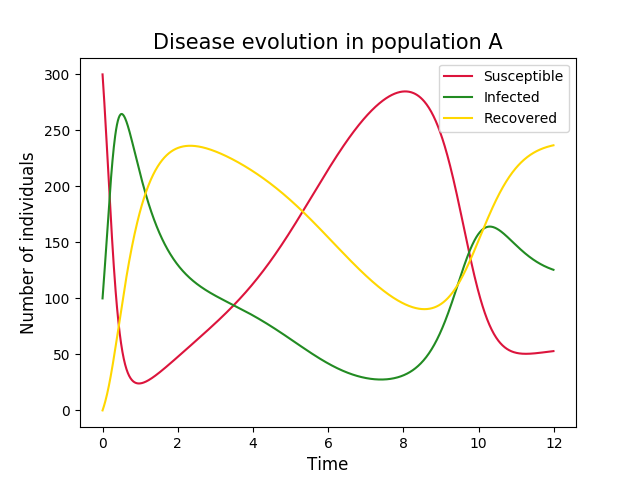
\includegraphics[width=0.45\textwidth]{../Figures/RK4_popA_sv}
	\caption{Time evolution of population A with vital a variable $a$, computed using RK4.}
	\label{RK4_sv}
\end{figure}
\begin{figure}
	\centering
	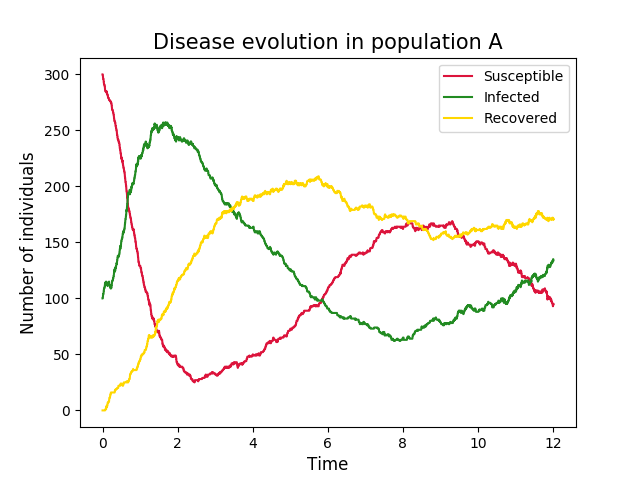
\includegraphics[width=0.45\textwidth]{../Figures/MC_popA_sv}
	\caption{Time evolution of population A with a variable $a$, computed using Monte Carlo.}
	\label{MC_sv}
\end{figure}
\begin{figure}
	\centering
	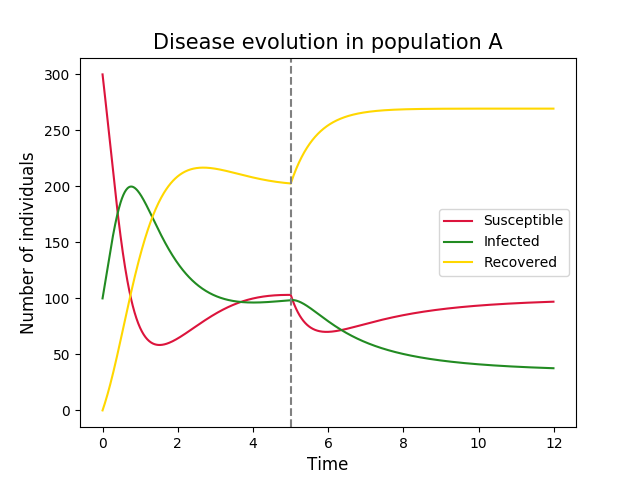
\includegraphics[width=0.45\textwidth]{../Figures/RK4_popA_vacc}
	\caption{Time evolution of population A, computed using RK4. The dashed line marks the start of vaccination.}
	\label{RK4_vacc}
\end{figure}
\begin{figure}
	\centering
	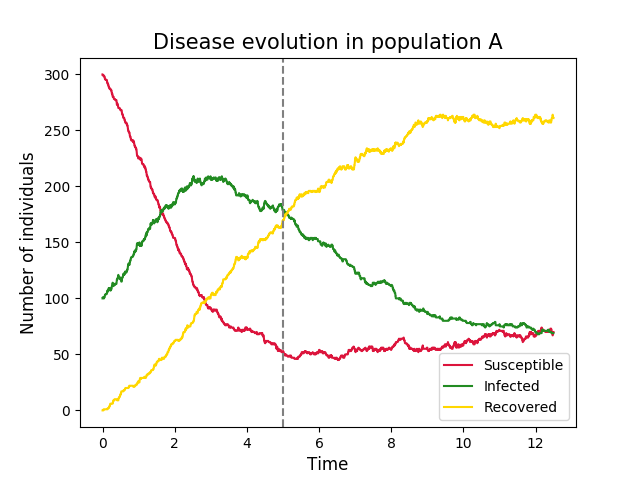
\includegraphics[width=0.45\textwidth]{../Figures/MC_popA_vacc}
	\caption{Time evolution of population A, computed using Monte Carlo. The dashed line marks the start of vaccination.}
	\label{MC_vacc}
\end{figure}
\begin{figure}
	\centering
	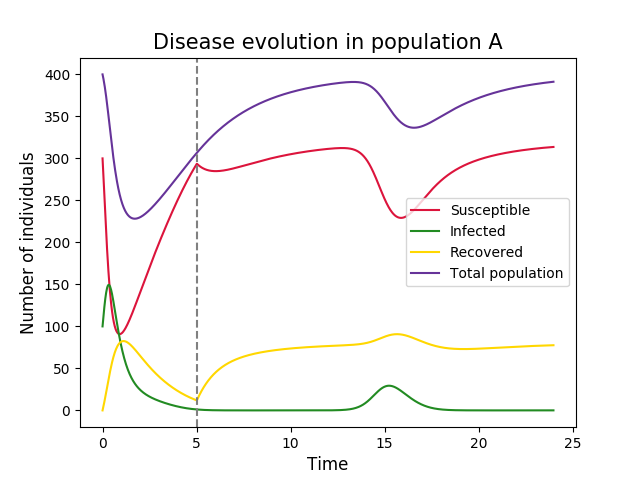
\includegraphics[width=0.45\textwidth]{../Figures/RK4_popA_combo}
	\caption{Time evolution of population A, computed using RK4. The dashed line marks the start of vaccination.}
	\label{RK4_combo}
\end{figure}
\begin{figure}
	\centering
	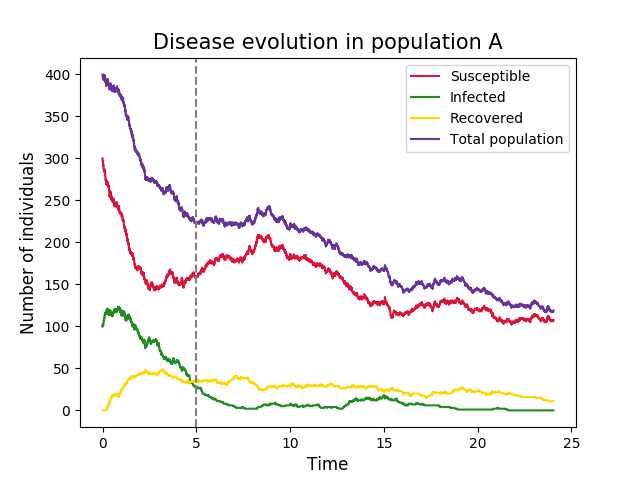
\includegraphics[width=0.45\textwidth]{../Figures/MC_popA_combo}
	\caption{Time evolution of population A, computed using Monte Carlo. The dashed line marks the start of vaccination.}
	\label{MC_combo}
\end{figure}

\clearpage
\section{Discussion}
In the basic model, we see that populations A and B both display a period of infection in the fourth order Runge-Kutta simulations (figures \ref{RK4_A} and \ref{RK4_B}). During this phase, the number of infected people increases. This phase only arises for these two populations because they have a low rate of recovery ($b$), meaning that people spend a longer time being infected (and infectious) before recovering, thus infecting a lot more people than in the other two populations. For populations C and D (figures \ref{RK4_C} and \ref{RK4_D}), the rate of recovery is so high that the number of infected people instantly sinks, leading to the eradication of the disease.\\[2mm]
We see these same patterns in the Monte Carlo simulations. However, the changes are slower and more gradual due to the random fluctuations.\\[2mm]
When vital dynamics are included for population A, neither the Runge-Kutta method nor the Monte Carlo method displays the same infection phase as seen in the basic model. Because of the high death rate of the disease, too many infected individuals die before they are able to infect a large number of people. An interesting difference between the two methods is the difference in evolution of total population. In the simulation using fourth order Runge-Kutta (figure \ref{RK4_vr}), the population starts with a dip (due to people succumbing to the disease) before it evens out to a nearly constant value around 350 people. The Monte Carlo simulation on the other hand, shows an increase in population size over time. The rate at which the population increases also gets higher over time. The rapid decrease of infected individuals found in the Runge-Kutta simulation is absent in the Monte Carlo simulation, where the decline of the disease is much slower.\\[2mm]
When it comes to the model including seasonal variation, we again see that the Monte Carlo simulation develops much slower than the fourth order Runge-Kutta simulation, and with less variation. \\[2mm]
The simulations of vaccinations again show similar trends to those seen above. The effect of the vaccination is immediately noticeable in the Runge-Kutta plot (figure \ref{RK4_vacc}), but very difficult to pinpoint in the Monte Carlo simulation. \\[2mm]
The figures showing the simulation of the full model have some interesting aspects. First of all, for the fourth order Runge-Kutta simulation of figure \ref{RK4_combo}, we see that there is a second small-scale outbreak happening late in the simulation due to the seasonal variation. This is only allowed to happen because we have a non-zero rate of immunity loss. This is what happens for viruses that evolve quickly and demonstrate a large genetic variety, such as the influenza virus.  However, the breakout remains small due to the high mortality rate and the vaccination which is happening concurrently with the breakout. \\[2mm]
The full model simulation using the Monte Carlo method looks very different from the Runge-Kutta simulation. Firstly, the second outbreak which is clearly visible in the Runge-Kutta plot is hardly visible. Secondly, and most worryingly when it comes to the quality of the model implementation, the population is decreasing. This is worrying because the birth rate is higher than the death rate, and the low number of infected people means that not many people are dying due to the disease. The deaths seem to be happening in the susceptible group, but why the deaths are so rapid is unclear.\\[2mm]
In general, all simulations show that the Monte Carlo simulations require longer time for large scale patterns to emerge. Changes to the population and disease development (such as seasonal variation or the start of vaccination) are harder to detect directly. Overall, the Runge-Kutta simulations are easier to interpret directly, although the Monte Carlo model might be more realistic in terms of disease transmission and discreteness.\\[2mm]
A weakness with the implementation shown is this report is that the disease and population data are not based on numbers from any real diseases or populations. Therefore, these specific simulations cannot be said to emulate any specific kind of disease.\\[2mm]
The model is explored for small populations, and future projects should look into how the model behaves for larger populations. In addition, the model should be compared to how real diseases are known to have spread in populations in order to determine it's ability to predict how diseases actually behave.

\section{Conclusion}
The aim of this project was to develop a Monte Carlo solution for the SIR-model, based on the differential solution method. The Monte Carlo solution produced was able to mimic the Runge-Kutta solution in most cases, albeit at a much slower pace. However, there were concerns about the quality of the method, particularly regarding the model including vital dynamics. In this case, the Monte Carlo method displayed a rapid increase or decrease in population, where the Runge-Kutta method was stable. \\[2mm]
Future projects should investigate the implementation of the method, particularly the implementation of vital dynamics. It would also be of interest to compare the model to known outbreaks in order to study its efficiency and ability to predict actual disease behaviour.



\onecolumngrid
\bibliographystyle{unsrtnat}
\bibliography{references.bib}










\end{document}